% (The MIT License)
%
% Copyright (c) 2023-2024 Yegor Bugayenko
%
% Permission is hereby granted, free of charge, to any person obtaining a copy
% of this software and associated documentation files (the 'Software'), to deal
% in the Software without restriction, including without limitation the rights
% to use, copy, modify, merge, publish, distribute, sublicense, and/or sell
% copies of the Software, and to permit persons to whom the Software is
% furnished to do so, subject to the following conditions:
%
% The above copyright notice and this permission notice shall be included in all
% copies or substantial portions of the Software.
%
% THE SOFTWARE IS PROVIDED 'AS IS', WITHOUT WARRANTY OF ANY KIND, EXPRESS OR
% IMPLIED, INCLUDING BUT NOT LIMITED TO THE WARRANTIES OF MERCHANTABILITY,
% FITNESS FOR A PARTICULAR PURPOSE AND NONINFRINGEMENT. IN NO EVENT SHALL THE
% AUTHORS OR COPYRIGHT HOLDERS BE LIABLE FOR ANY CLAIM, DAMAGES OR OTHER
% LIABILITY, WHETHER IN AN ACTION OF CONTRACT, TORT OR OTHERWISE, ARISING FROM,
% OUT OF OR IN CONNECTION WITH THE SOFTWARE OR THE USE OR OTHER DEALINGS IN THE
% SOFTWARE.

\documentclass{article}
\usepackage{../lecture-notes/notes}
\newcommand*\thetitle{Builds}
\begin{document}

\plush{\lnTitlePage{21}{24}{QQUda0fAcxE}}

\lnQuote
  [Grady Booch]
  {grady-booch}
  {In general, there may be more internal releases to the development team, with only a few executable releases turned over to external parties. The internal releases represent a sort of \ul{continuous integration} of the system and exist to force closure on some key system areas.}
  {booch1994object}

\lnQuote
  [Michael Cusumano]
  {michael-cusumano}
  {Regardless of how often individual developers check in their changes to the source code, a designated developer, called the project \ul{build master}, generates a complete build of the product on a daily basis using the master version of the source code.}
  {cusumano1997microsoft}

\lnQuote
  {../21-builds/msft}
  {[In Microsoft], the rule is that if developers check in code that `breaks' the \ul{build} by preventing it from completing the \ul{recompilation}, they must fix the defect \ul{immediately}.}
  {cusumano1997microsoft}

\lnQuote
  [Kent Beck]
  {kent-beck}
  {Developers need freedom to make changes where they make the most sense. Therefore, \ul{integrate} and \ul{test} several times a day. Throw away unintegrated code after a couple of days and start over. Ignore code ownership. Program in pairs. Don't integrate \ul{without unit tests}.}
  {beck1998extreme}

\lnQuote
  [Martin Fowler]
  {martin-fowler}
  {For most projects, the XP guideline of a \ul{ten minute} build is perfectly within reason. Most of our modern projects achieve this. It's worth putting in concentrated effort to make it happen, because every minute chiseled off the build time is a minute \ul{saved} for each developer every time they commit.}
  {fowler2006}

\lnQuote
  [Jez Humble]
  {jez-humble}
  {Automation is the key. It allows all of the \ul{common tasks} involved in the creation and deployment of software to be performed by developers, testers, and operations personnel, at the \ul{push of a button}.}
  {humble2010continuous}

\lnQuote
  [Bogdan Vasilescu]
  {bogdan-vasilescu}
  {Our main finding is that continuous integration improves the \ul{productivity} of project teams, who can integrate \ul{more} outside contributions, without an observable diminishment in \ul{code quality}.}
  {vasilescu2015quality}

\lnQuote
  [Kai Huang]
  {kai-huang}
  {Our results show there are good reasons for the rise of CI. Compared to projects that do not use CI, projects that use CI: \ul{release} twice as often, \ul{accept pull requests} faster (1.6x), and have developers who are \ul{less worried} about breaking the build.}
  {hilton2016usage}
\lnPitch{\begin{multicols}{2}
  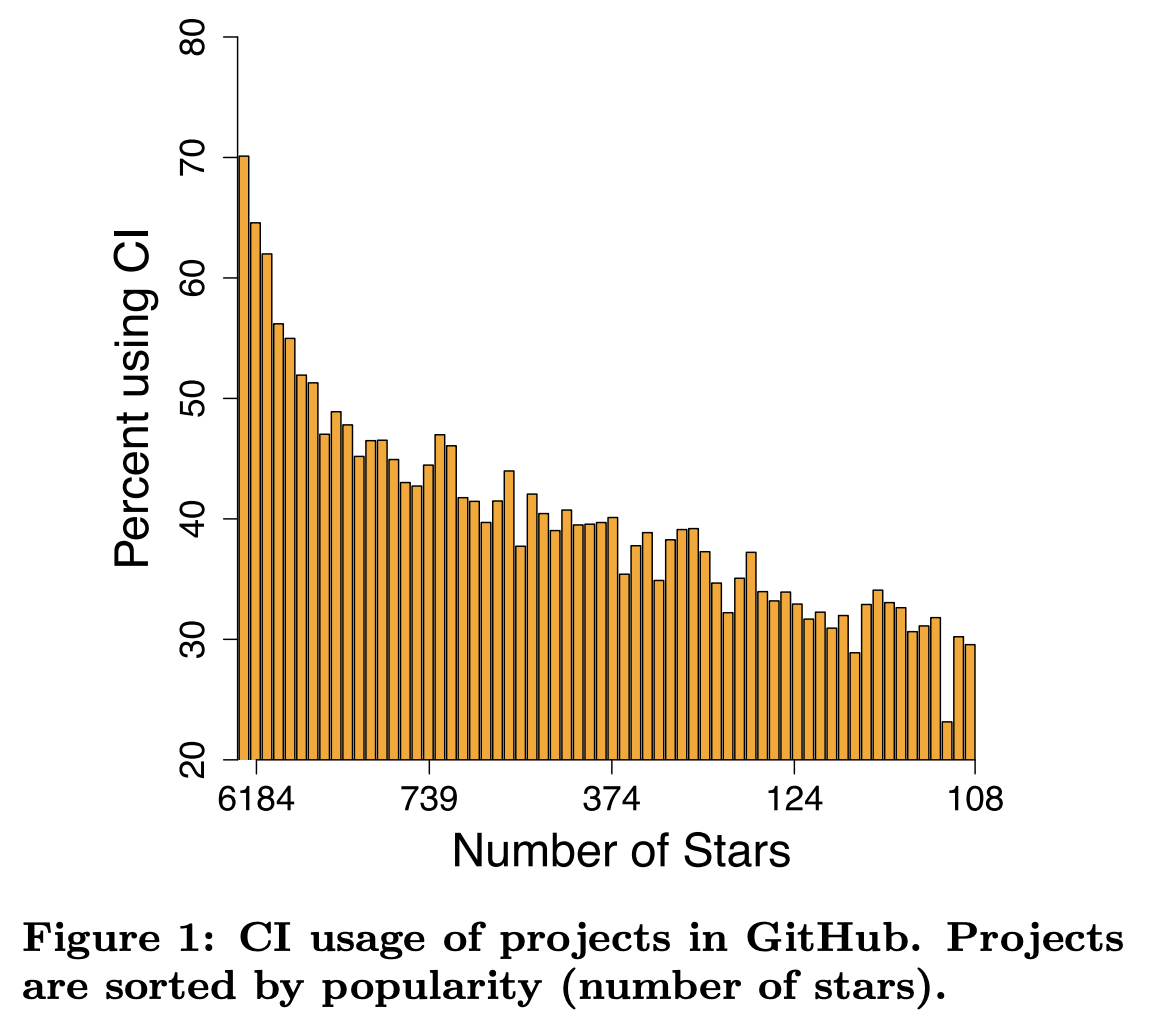
\includegraphics[width=.9\linewidth]{by-stars.png}
  \par\columnbreak\par
  ``In the most popular (starred) group, 70\% of projects use CI. As the projects become less popular, the percentage of projects using CI declines to 23\%. Observation: Popular projects are more likely to use CI.''
  \lnSource{hilton2016usage}
  \end{multicols}}
\lnPitch{\begin{multicols}{2}
  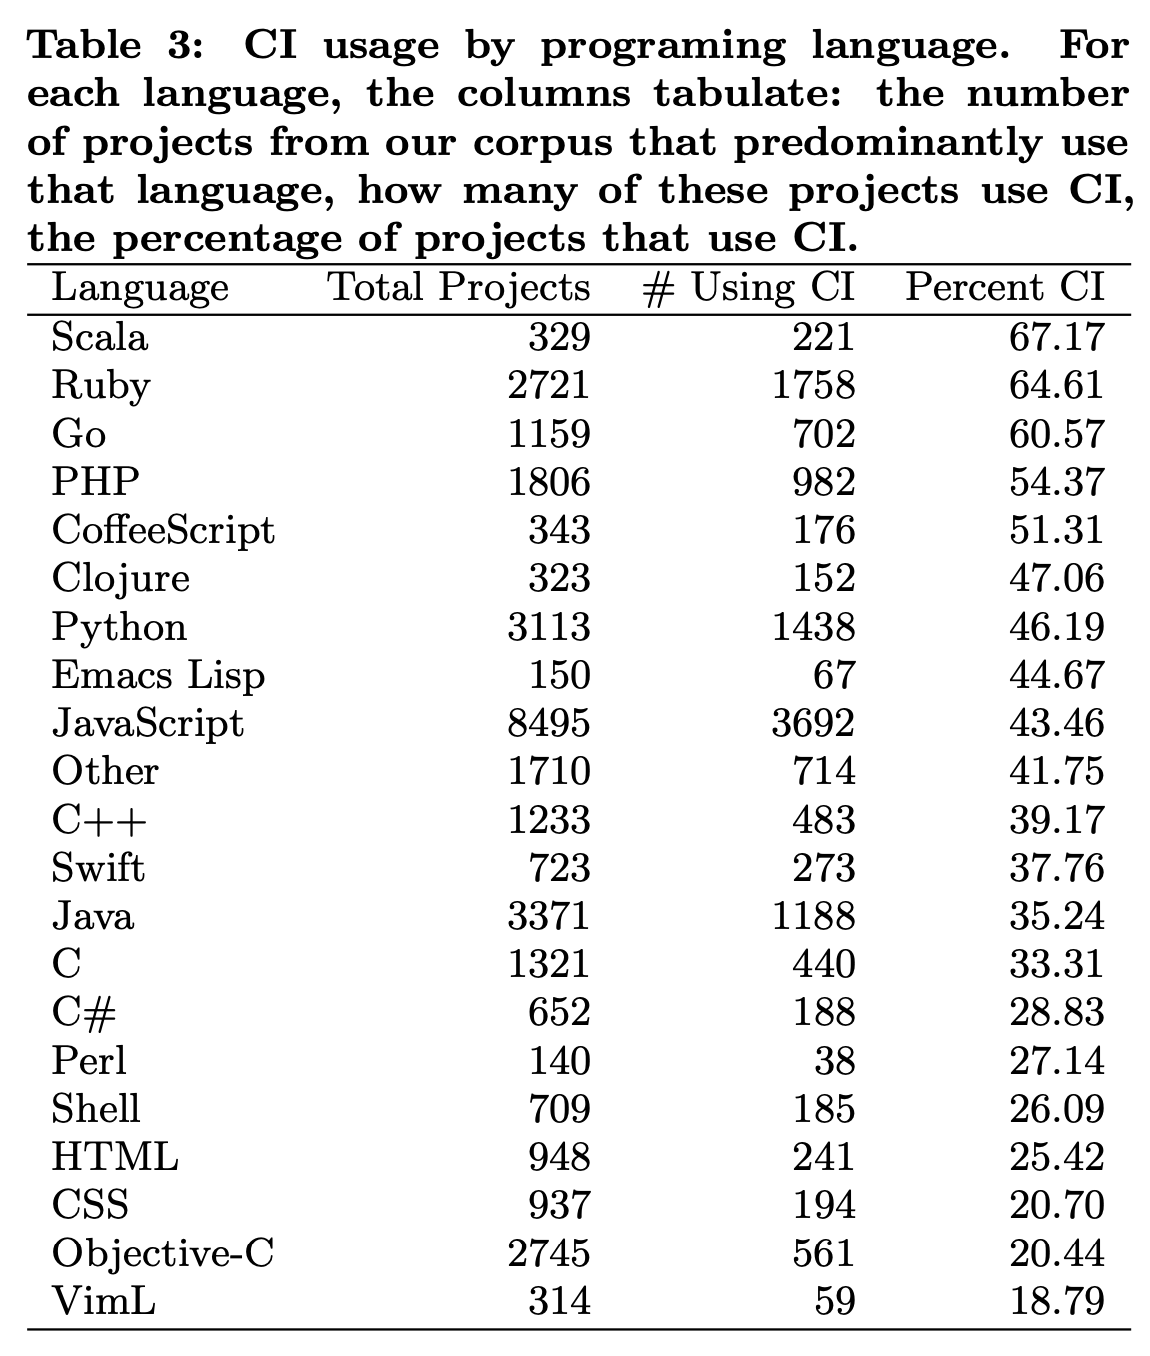
\includegraphics[width=.8\linewidth]{by-language.png}
  \par\columnbreak\par
  ``Languages that have the highest CI usage are also dynamically-typed (e.g., Python and JavaScript). One possible explanation may be that in the absence of a static type system which can catch errors early on, these languages use CI to provide extra safety.''
  \lnSource{hilton2016usage}
  \end{multicols}}
\lnPitch{\begin{multicols}{2}
  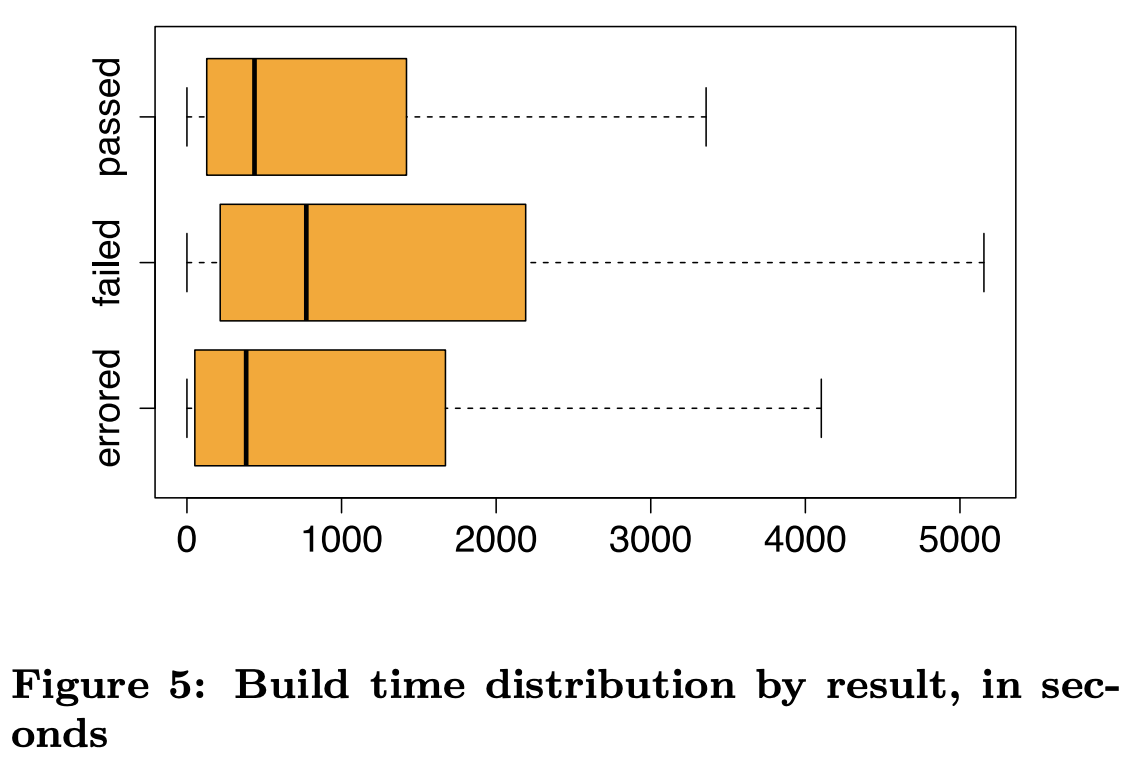
\includegraphics[width=.9\linewidth]{duration.png}
  \par\columnbreak\par
  ``The average build time is just under 500 seconds. Errored builds are those that occur before the build begins (e.g., when a dependency cannot be downloaded), and failed builds are those that the build is not completed successfully.''
  \lnSource{hilton2016usage}
  \end{multicols}}

\lnQuote
  [Michael Hilton]
  {michael-hilton}
  {Developers use CI to guarantee \ul{quality}, consistency, and viability across different environments. However, adding and maintaining automated tests causes these benefits to come at the expense of \ul{increased time} and \ul{effort}.}
  {hilton2017trade}
\lnPitch{\begin{multicols}{2}
  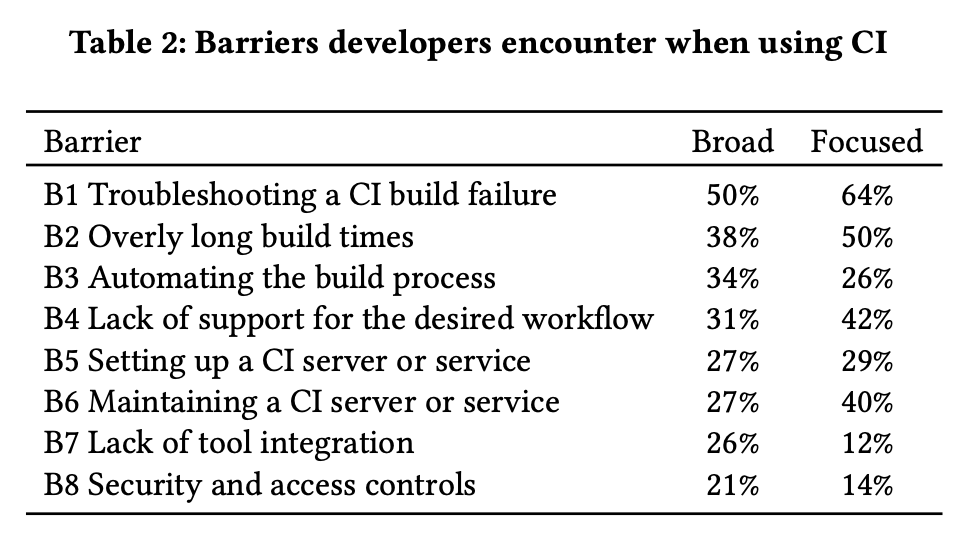
\includegraphics[width=.9\linewidth]{barriers.png}
  \par\columnbreak\par
  ``When a CI build fails, some participants begin the process of identifying why the build failed. \ul{Sometimes}, this can be fairly straightforward...''
  \lnSource{hilton2017trade}
  \end{multicols}}
\lnPitch{\begin{multicols}{2}
  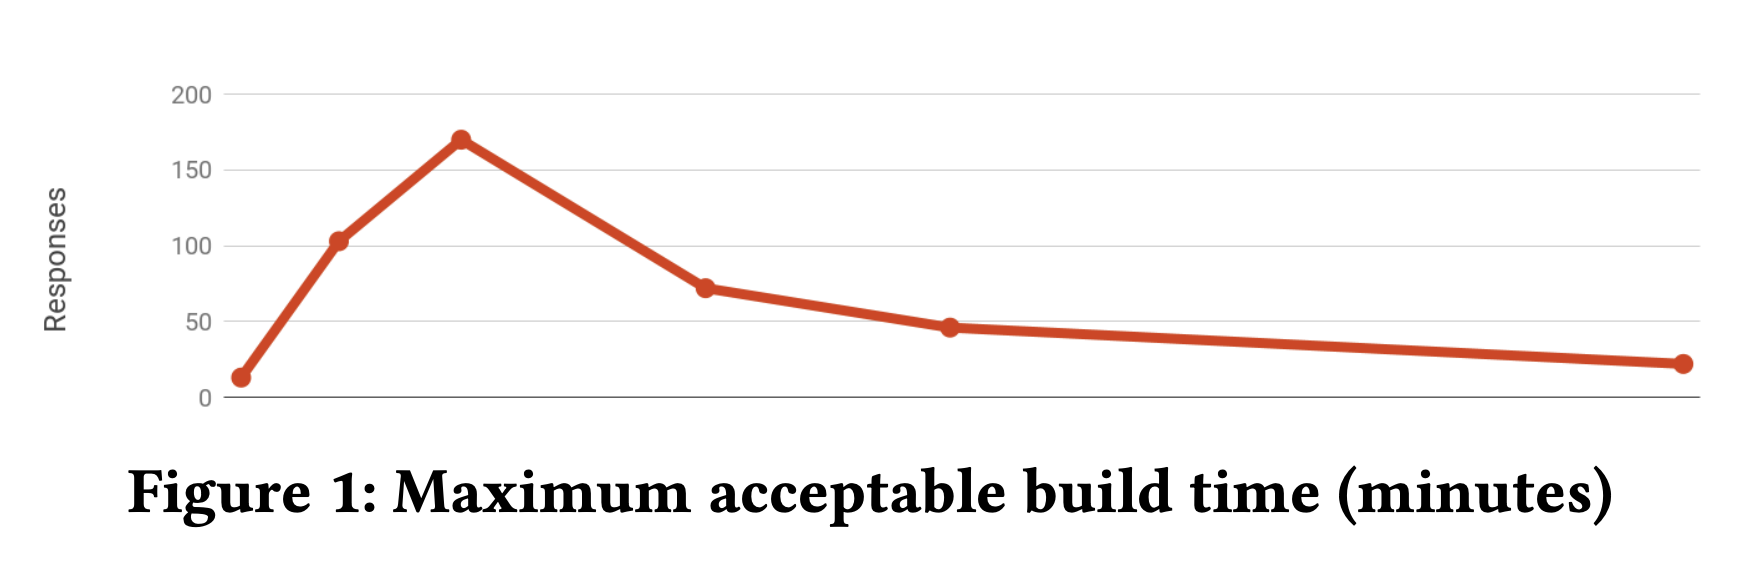
\includegraphics[width=.9\linewidth]{ten-minutes.png}
  \par\columnbreak\par
  ``\citep{fowler2006} suggests most projects should try to follow the XP guideline of a 10-minute build. When we asked our 523 participants what is the \ul{maximum acceptable time} for a CI build to take, the \ul{most common answer} was also 10 minutes.''
  \lnSource{hilton2017trade}
  \end{multicols}}
\lnPitch{\begin{multicols}{2}
  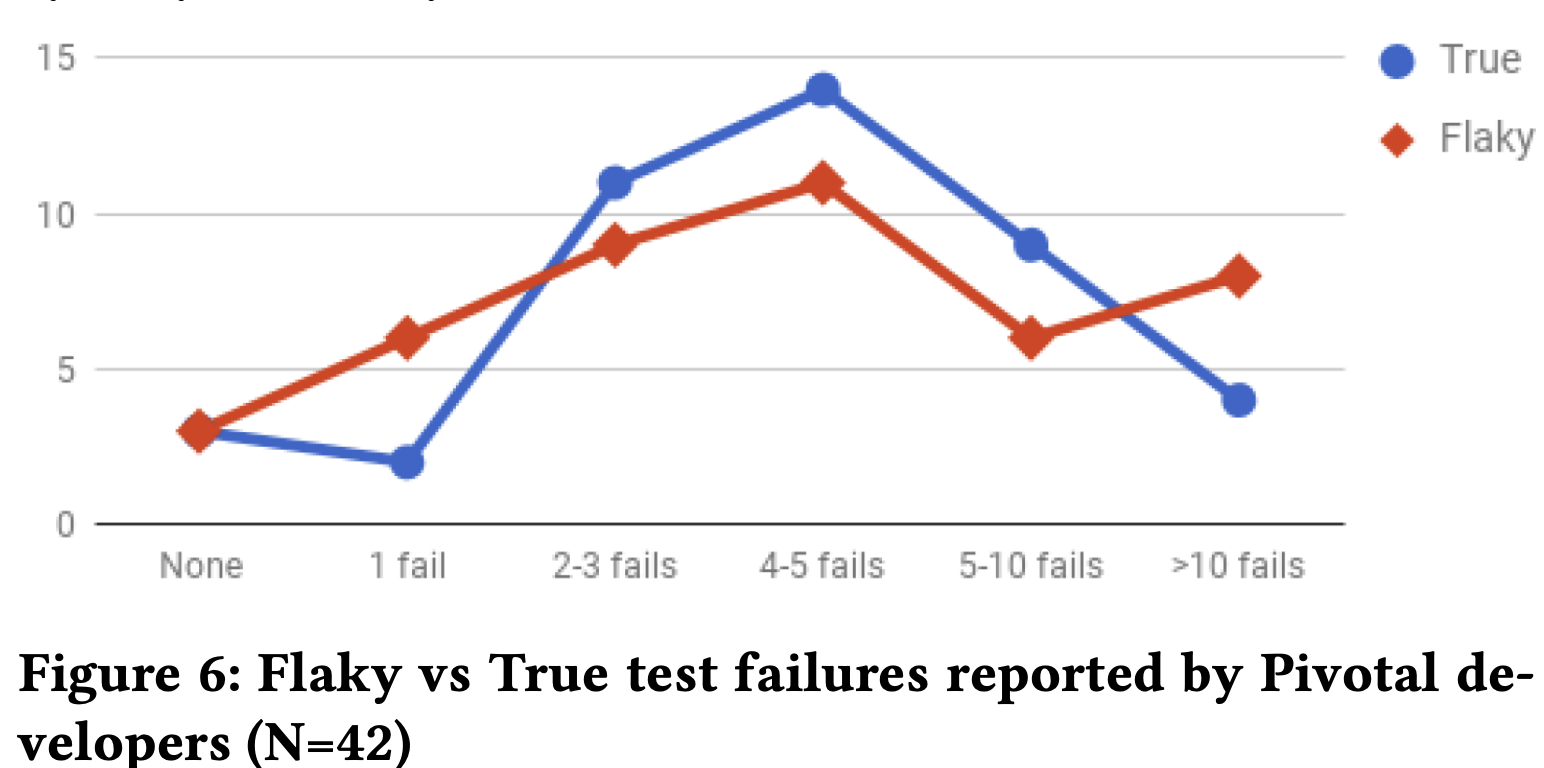
\includegraphics[width=.9\linewidth]{flaky.png}
  \par\columnbreak\par
  ``Pivotal developers experienced similar numbers of flaky and true CI failures per week. However, for the largest category, \ul{>10 fails a week}, there were twice as many flaky failures as true failures.''
  \lnSource{hilton2017trade}
  \end{multicols}}

\lnQuote
  [John Micco]
  {john-micco}
  {Unfortunately, across our entire corpus of tests, we [in Google] see a continual rate of about 1.5\% of \ul{all test runs} reporting a `flaky' result.}
  {micco2016}
\plush{\pptBanner{Google Thoughts About Flaky Tests}
  \begin{itemize}
  \item Almost 16\% of our 4.2M tests have some level of flakiness
  \item 84\% of transitions from Pass -> Fail are from `flaky' tests
  \item We spend up to 16\% of our compute resources re-running flaky tests
  \item Certain people/automation more likely to cause breakages (oops!)
  \item Certain languages more likely to cause breakages (sorry)
  \end{itemize}
  \lnSource{micco2017state}}

\lnQuote
  [Carmine Vassallo]
  {carmine-vassallo}
  {In total, the 349 projects underwent 116,741 builds, of which 30,792 (26\%) failed. It is interesting to notice how the percentage of build failures is approximately the same in OSS and ING.}
  {vassallo2017tale}

\lnQuote
  [Thomas Rausch]
  {thomas-rausch}
  {Process metrics have a significant impact on the build outcome in 8 of the 14 projects on average, but the strongest influencing factor across all projects is \ul{overall stability} in the \ul{recent build history}. For 10 projects, more than 50\% (up to 80\%) of all failed builds follow a previous build failure.}
  {rausch2017empirical}
\lnPitch{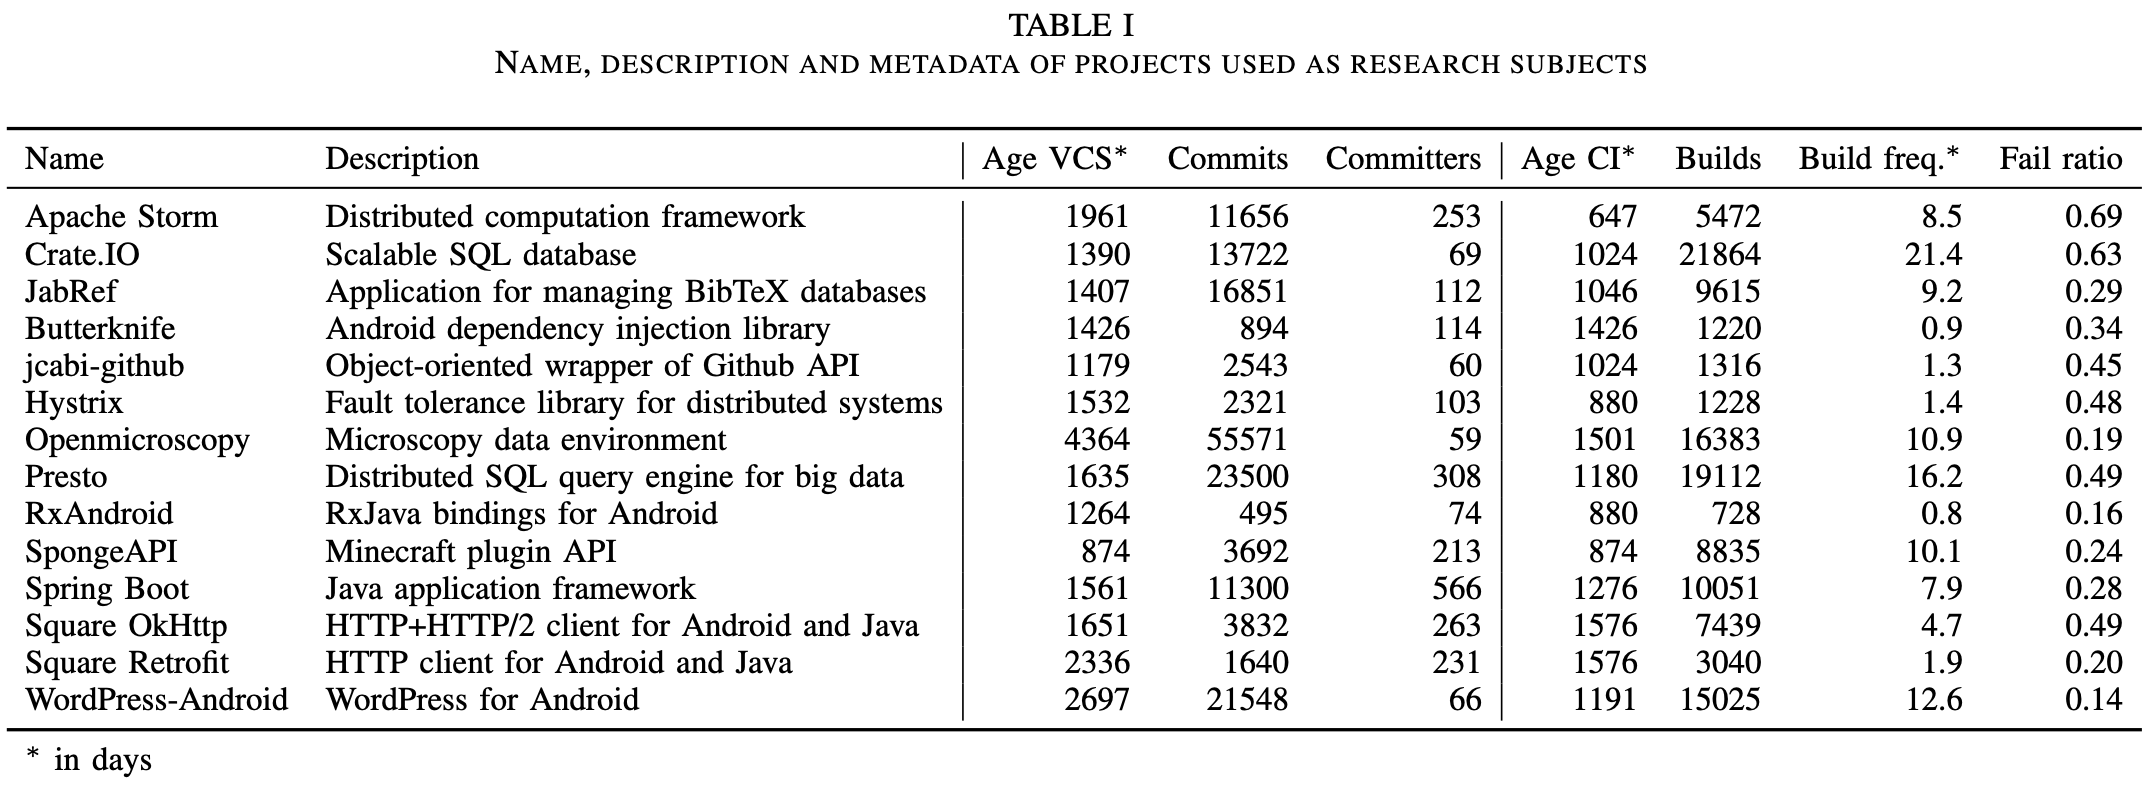
\includegraphics[width=.9\linewidth]{fail-ratio.png}
  \par
  \lnSource{rausch2017empirical}}
\lnPitch{\begin{multicols}{2}
  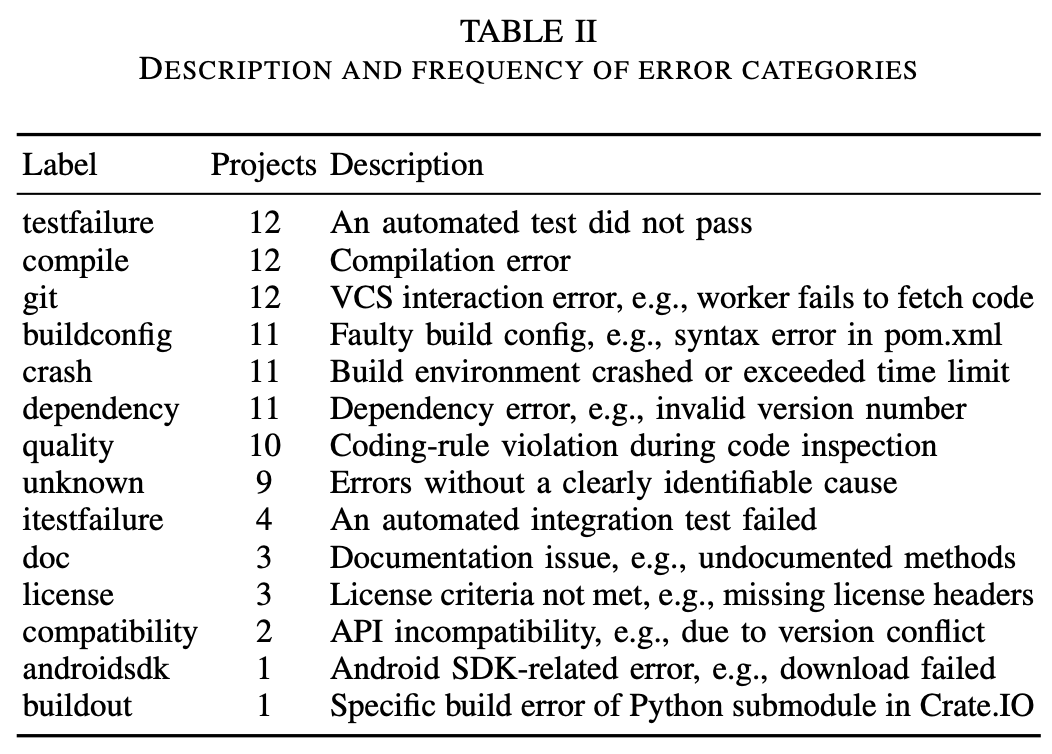
\includegraphics[width=.9\linewidth]{error-types.png}
  \lnSource{rausch2017empirical}
  \par\columnbreak\par
  ``On average, 41\% of builds fail because of test failures... On average, 30\% of errors occur in the first half of the build runtime. The later half is dominated by 70\% testfailures. Together with a build-retry approach, testfailures can cause long delays in the feedback loop.''
  \end{multicols}}

\lnQuote
  [Romit Jain]
  {romit-jain}
  {We observed that team size generally \ul{increases} the number of build failures. The interesting observation here is the minima after which there is a positive curve.}
  {jain2018brief}
\lnPitch{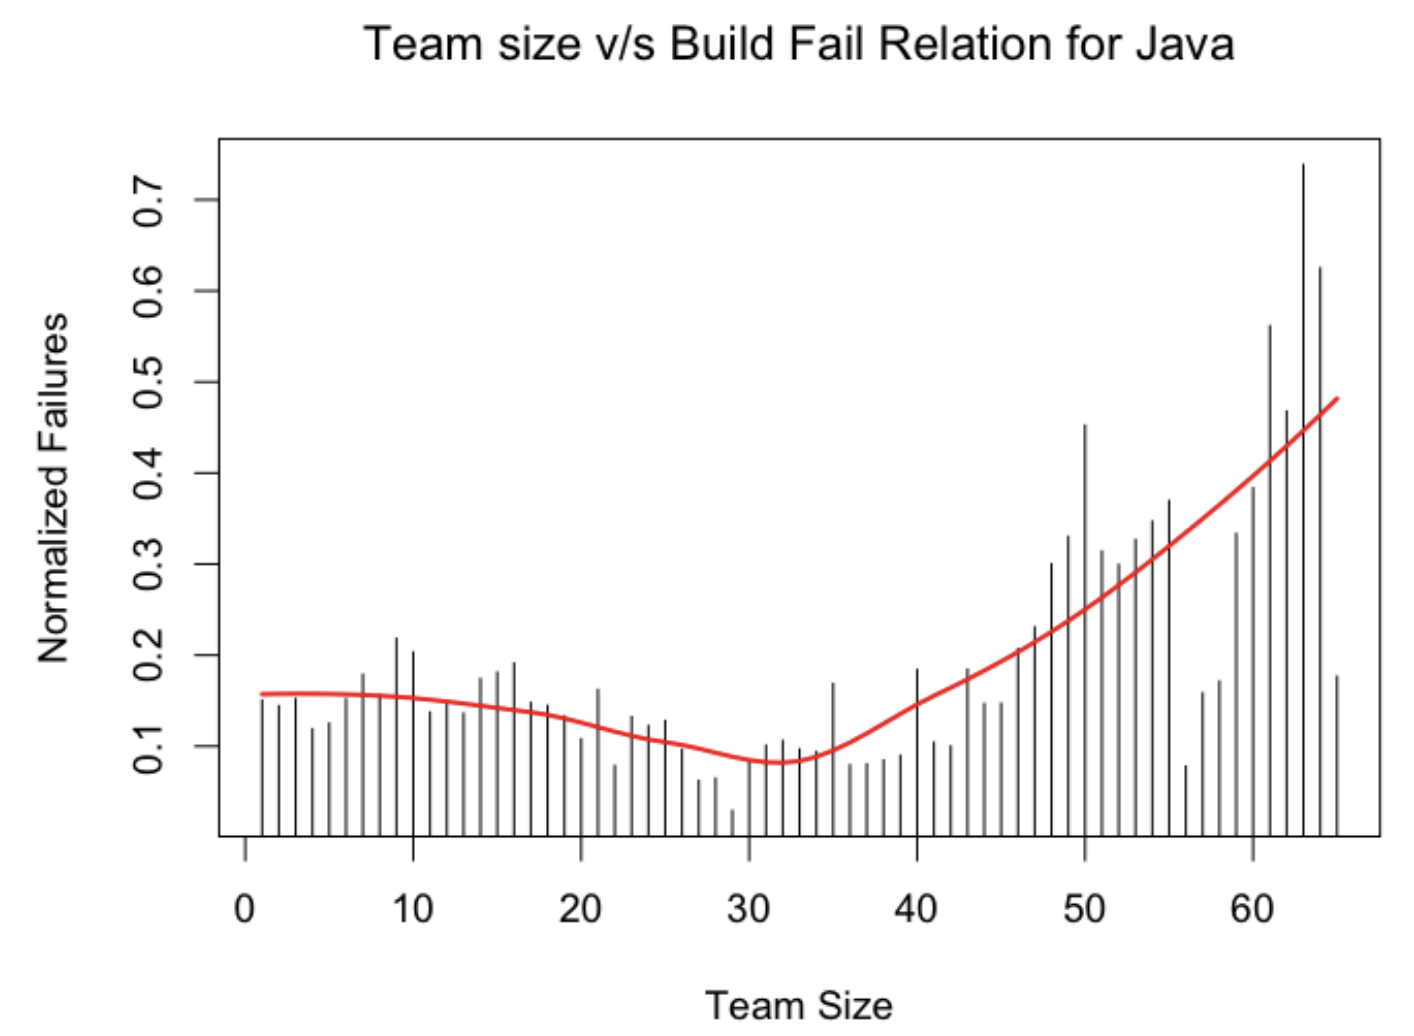
\includegraphics[width=.5\linewidth]{team-size.png}
  \lnSource{jain2018brief}}
\lnPitch{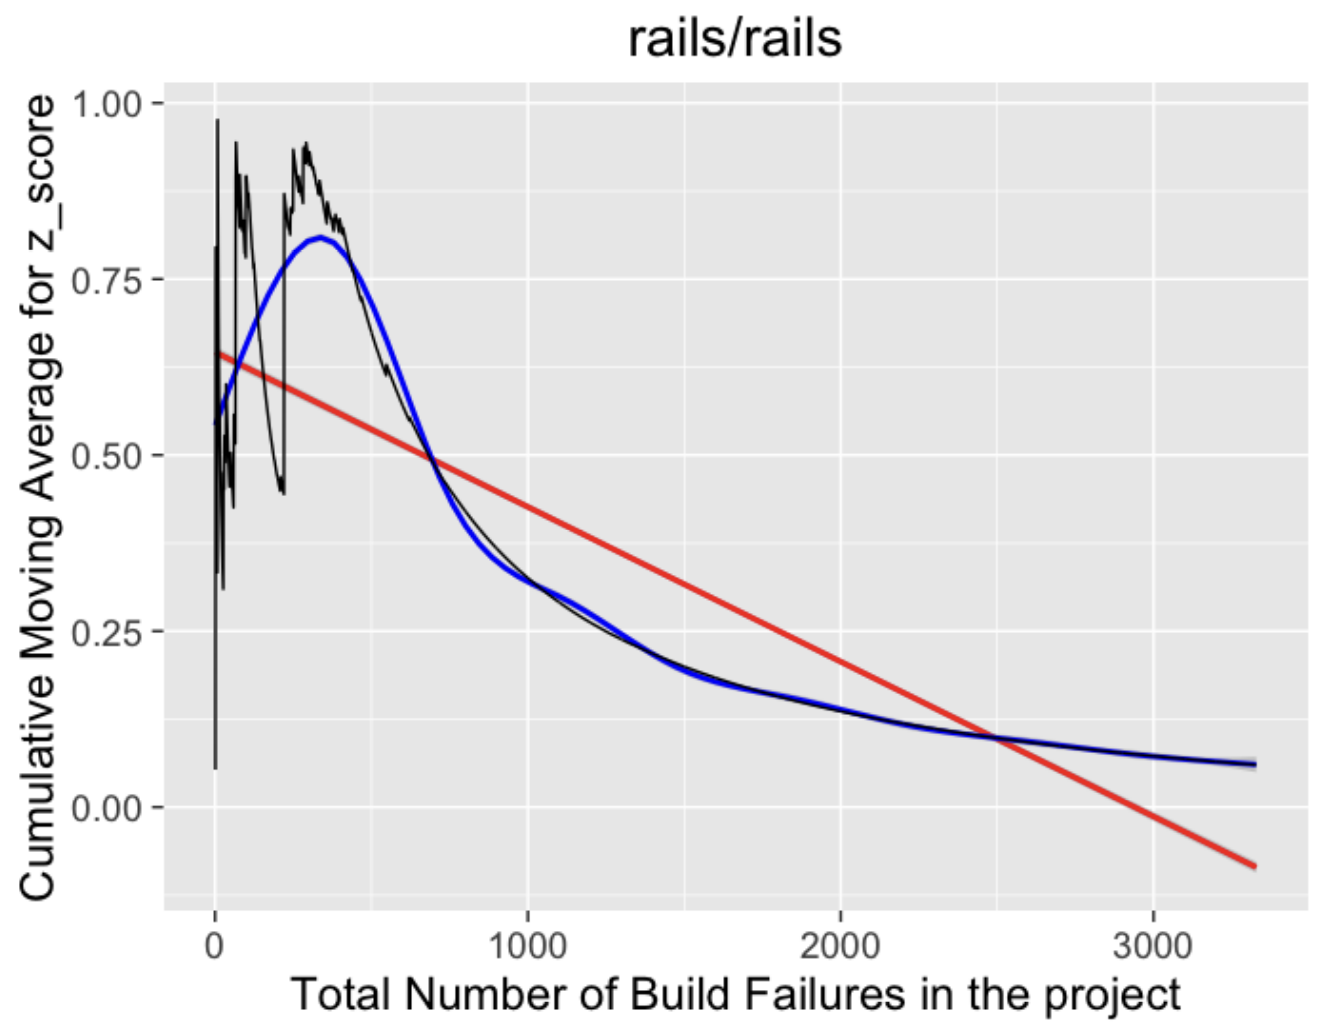
\includegraphics[width=.5\linewidth]{productivity.png}
  \lnSource{jain2018brief}}

\plush{\pptThought{\href{}{On October 16, 2018}, \newline GitHub launched ``Actions''}}

\lnQuote
  [Mehdi Golzadeh]
  {mehdi-golzadeh}
  {Together with Travis, GHA covers more than 80\% of all usages. Moreover, in only 18 months GHA has overtaken all other CIs in popularity.}
  {golzadeh2022rise}
\lnPitch{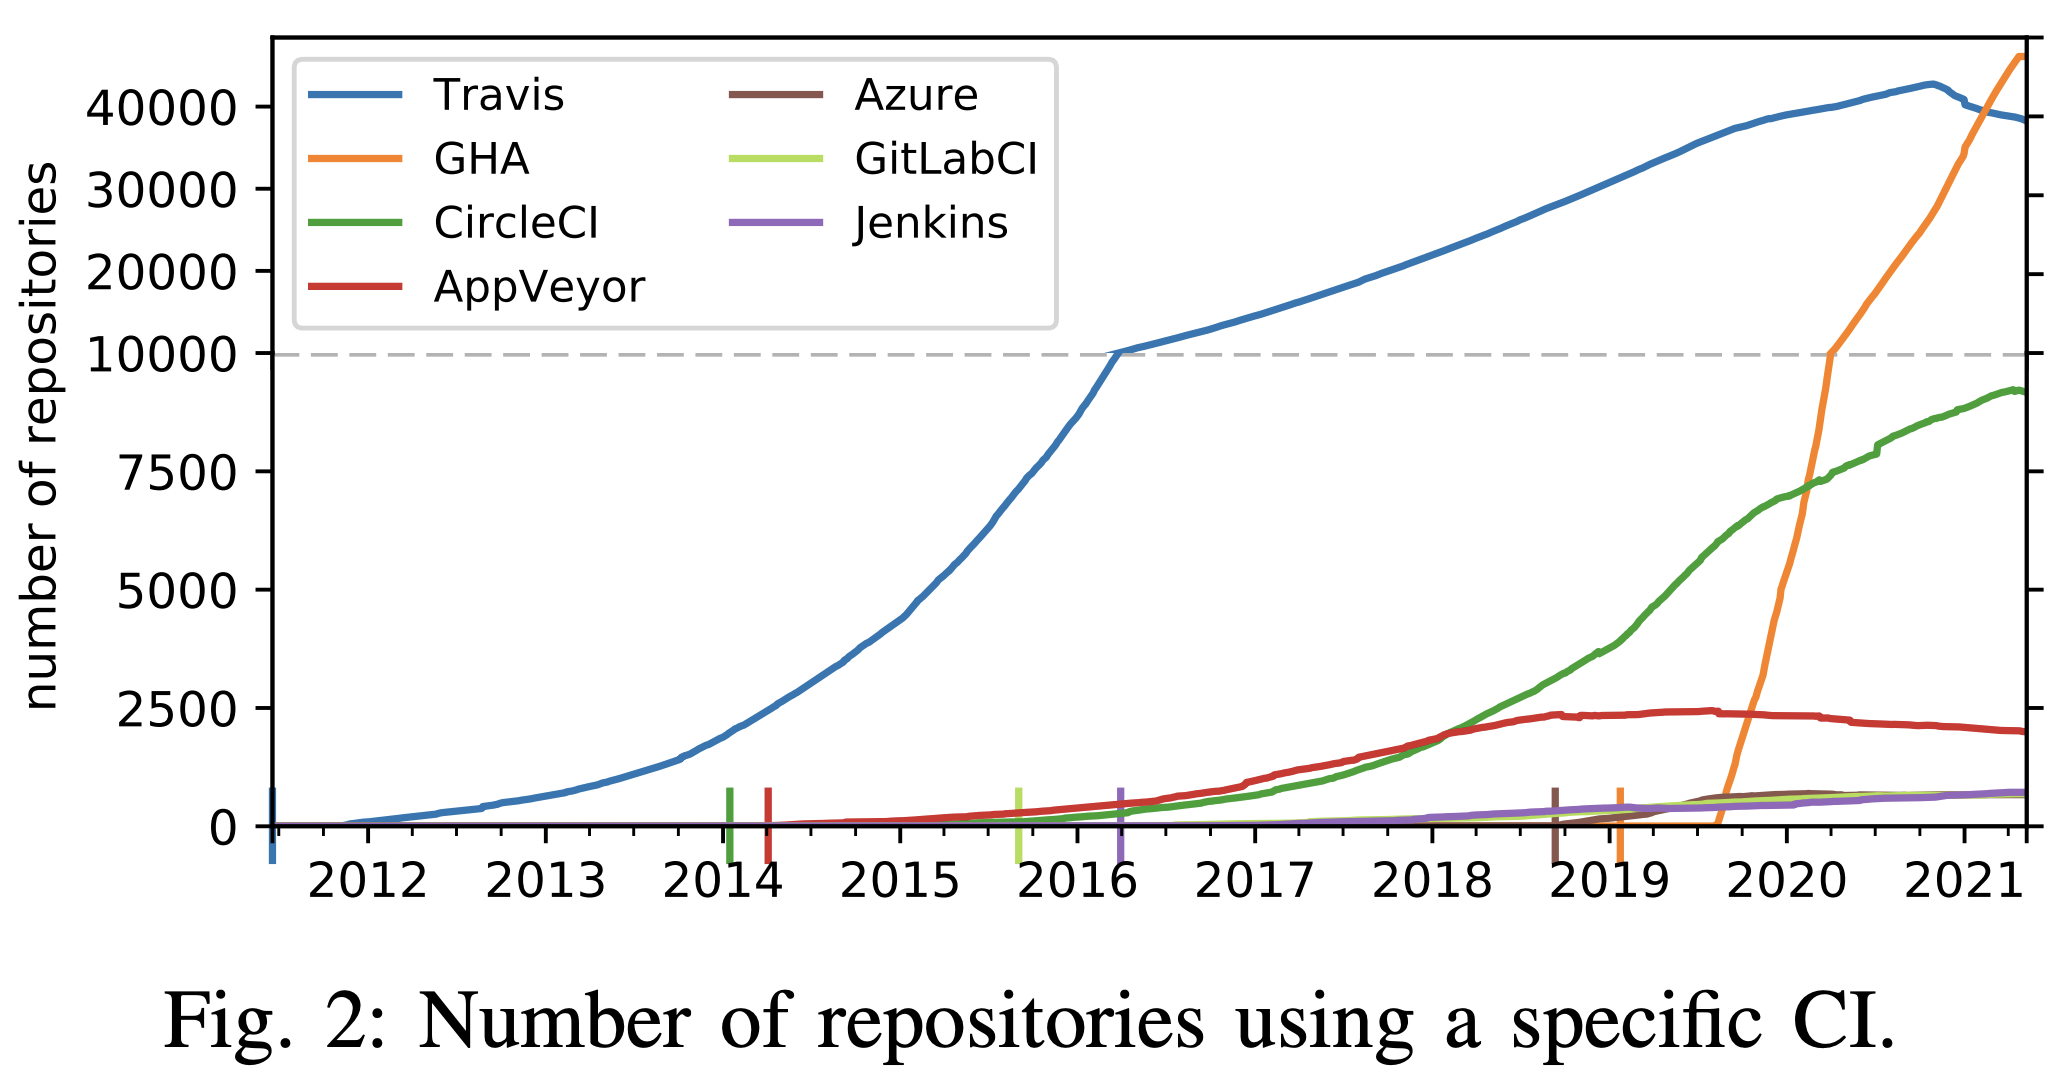
\includegraphics[width=.75\linewidth]{gha-growth.png}
  \lnSource{golzadeh2022rise}}

\lnQuote
  [Wing Lam]
  {wing-lam}
  {We find that \ul{53\%} of flaky tests detected in CI runs are not detected in isolation.}
  {lam2020understanding}

\lnQuote
  [Owain Parry]
  {owain-parry}
  {The causes and associated factors of flaky tests: \begin{enumerate*}
    \item Asynchronicity and Concurrency,
    \item Platform Dependencies,
    \item Floating-Point numbers,
    \item Order-dependent tests,
    \item Unordered Collections,
    \item Shared access to static fields,
    \item Timeouts,
    \item I/O and Network,
    \item Algorithmic Non-determinism.
  \end{enumerate*}}
  {parry2021survey}

\lnQuote
  [Pei Liu]
  {pei-liu}
  {We start by collecting a set of 84,475 open-source Android apps from the most popular three online code hosting sites, namely Github, GitLab, and Bitbucket. We then look into those apps and find that only around 10\% of apps have leveraged CI/CD services, i.e., the \ul{majority} of open-source Android apps are developed \ul{without} accessing CI/CD services.}
  {liu2022first}

\lnQuote
  [Shanto Rahman]
  {shanto-rahman}
  {FlakeSync works by \ul{identifying} a critical point, representing some key part of code that must be executed early w.r.t. other concurrently executing code, and a barrier point, representing the part of code that should wait until the critical point has been executed. FlakeSync can \ul{modify} code to check when the critical point is executed and have the barrier point keep waiting until the critical point has been executed, essentially synchronizing these two parts of code for the specific test execution.}
  {rahman2024flakesync}

\end{document}
